\documentclass[a4paper,10pt]{article}
\usepackage[utf8]{inputenc}
\usepackage{graphicx}
\usepackage{url}
\usepackage{float}
\usepackage{times}
\usepackage{multirow}
\usepackage{listings}
\usepackage{times}
\usepackage{paralist}
\usepackage{epsfig}
\usepackage{subfigure}
\usepackage[hypertex]{hyperref}
\usepackage{subfigure}
\usepackage{color}

%\documentclass{rspublic}

\usepackage{ifpdf}
\newcommand{\athotanote}[1]{ {\textcolor{green} { ***athota: #1 }}}

\newcommand{\I}[1]{\textit{#1}}
\newcommand{\B}[1]{\textbf{#1}}
\newcommand{\BI}[1]{\textbf{\textit{#1}}}
\newcommand{\T}[1]{\texttt{#1}}

\setlength\topmargin{0in}
\setlength\headheight{0in}
\setlength\headsep{0in}
\setlength\textheight{9in}
\setlength\textwidth{6.5in}
\setlength\oddsidemargin{0in}
\setlength\evensidemargin{0in}
\setlength\parindent{0.1in}
\setlength\parskip{0.25em}


\ifpdf
 \DeclareGraphicsExtensions{.pdf, .jpg}
\else
 \DeclareGraphicsExtensions{.eps, .ps}
\fi

\newcommand{\note}[1]{ {\textcolor{red} { ***NOTE: #1 }}}

\begin{document}

\title{\LARGE Running Asynchronous Replica-Exchange Simulations Across Heterogeneous Distributed Infrastructures}
 
\author{Shantenu Jha$^{1,2,3}$, Abhinav Thota$^{1,2}$, Andre Luckow$^{1}$ \\
   \small{\emph{$^{1}$Center for Computation \& Technology, Louisiana State University, USA}}\\
   \small{\emph{$^{2}$Department of Computer Science, Louisiana State University, USA}}\\
   \small{\emph{$^{3}$e-Science Institute, University of Edinburgh, UK}}
   }
 
\maketitle
 
Writing applications that are able to orchestrate heterogeneous
resources across virtual organizations (VO) is a complex task.  Several 
classes of applications, which are well suited for loosely
coupled Grids, exist; arguably the best known and most commonly used ones are
task farming applications. Despite the simple nature, many problems
can be solved with such a model, e.\,g.\ parameter studies found in
many sciences or Monte Carlo simulations. More complicated, but possibly more 
interesting than {\it pleasingly  distributed} applications, is the class of applications that are
essentially loosely-coupled, but with a small level of coupling
between the tasks.  A class of algorithms that belongs to this category are
\emph{Replica Exchange Molecular Dynamics (REMD)}~\cite{hansmann,Sugita:1999rm} simulations. 
 
 
- 1 para intro to replica-exchange, and how it is traditionally done (ie case I)
Previously, adaptive distributed replica-exchange simulations were carried out using the BigJob abstraction.~\cite{Luckow et al. 2009}
 Depending on the number of processes n, the manager created n/2 pairs of replicas. Before launching a job, the manager
 ensured that all required input files are transferred to the respective
resource. For this purpose, the SAGA File API and the GRIDFTP adaptor were
used. The replica jobs were then submitted to the resource using the SAGA CPR
API and the MIGOL/GRAM middleware.
When all replicas reached a pre-determined state (e.g. the NAMD job finishes
after a fixed number of steps), the decision as to whether to pairwise exchange
temperatures between neighbouring replicas was determined by the METROPOLIS
scheme. The run of an ensemble of replicas in parallel and the subsequent
pairwise exchange attempt are referred to as generation. No two replicas can
belong to different generations. If the exchange attempt was successful, parameters
such as the temperature were swapped. Both jobs were then relaunched. 
 \athotanote{I have tried to put here how the adaptive repex was done, supposing that it was case 1. Or should a general
  explanation of a replica exchange be here?}
 
- 1 para limitation on traditional replica exchange
The major limitation of this model is that the replicas are paired and the exchanges can only take place within those pairs. 
This limits the group of replicas which are available for exchange drastically. Moreover, the replicas are stuck with their partners, 
sometimes waiting for them to complete while there are possibly other replicas available which are paired to their partners.
This puts a strain on the number of exchanges that can take place within a certain time.
\athotanote{is it better to have a wide group of replicas?  need some input here!}

- Introduce asynchrononous Replica Exchange --  1 para on case II and case
III (algorithmically)
To overcome these limitations we are proposing a new mechanism where the replicas will have freedom to perform an exchange
with any other replica available, asynchronously. Again, we are going to be using the BigJob abstraction
and SAGA. \athotanote{is something more required here?}
We are implementing this in two ways.
The first is a centralized mechanism where all the replicas are managed by a master. The master will closely
monitor the replicas and will make the exchanges when feasible. 
The second is a decentralized mechanism where each replica is on its own and a wrapper script will perform the
the required actions to look for partners and will make the exchange.

- Describe how we implement Case II and Case III (you can use figures)
  using SAGA and the advantages
\section{Implementation}
Case 2: 
We are calling the centralized version of the replica exchange case 2. In this case, one or more BigJobs are
launched and the replicas are submitted to the BigJobs as and when they become active. The master, which also launches the BigJob,
now monitors the replicas. When a replica is done running, the master will start a search for an appropriate partner from all the available replicas. The matching mechanism
that is being used here is the Metropolis scheme. The energies of the two replicas which are negotiating an exchange are compared and a decision is reached.
Whether or not a successful exchange was possible, the master again monitors the replicas and when it finds a replica which has finished running, it tries to find it a partner.
After each successful exchange the replicas are resubmitted to the BigJob(s) and restarted.

Case 3:
Case 3 is the decentralized version. In this case, similar to the above case, one or more BigJobs are launched but instead of submitting the replicas as sub-jobs, the sub-job now is a wrapper script inside which is the replica. The script then launches the replica as the sub-job and monitors the replica and looks for partners to exchange as and when the replica is done. In this case the too the various functions needed to make the exchange are carried out by the wrapper script. In this case the replicas will only have to restarted but not resubmitted to the BigJob(s). The temperatures, energies and states of a replica are reported to and retrieved from the SAGA advert service in real-time.

%%%%% FIGURE %%%%%
\begin{figure}
\centering
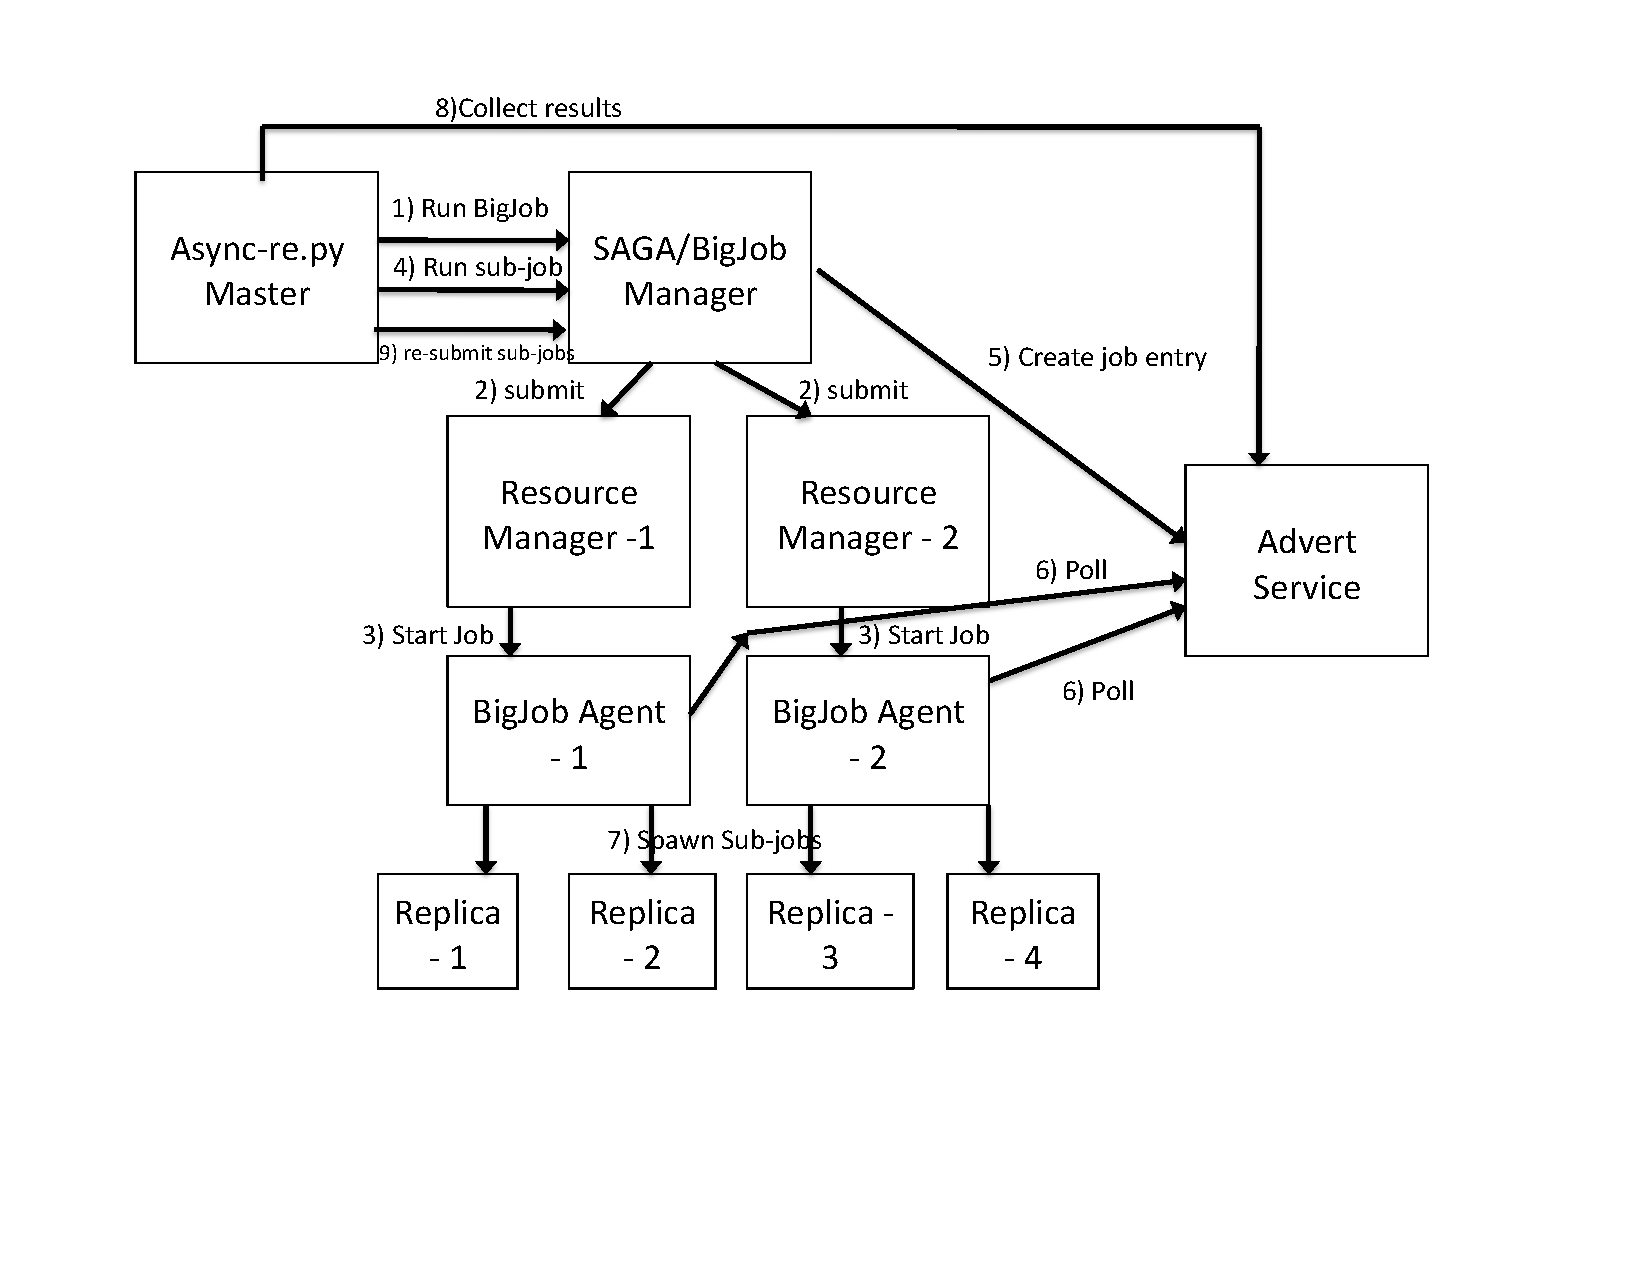
\includegraphics[scale=0.50]{centralized_architecture.pdf}
\caption{\small Centralized}
\label{Fig:Centralized}
%\vspace{-1em}
\end{figure}
%%%%% FIGURE %%%%%

%%%%% FIGURE %%%%%
\begin{figure}
\centering
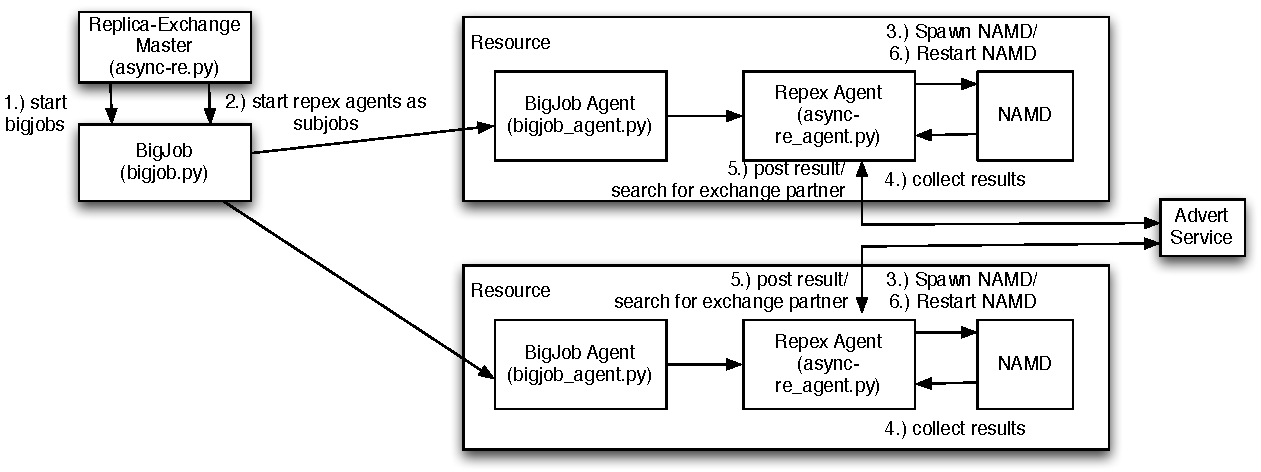
\includegraphics[scale=0.50]{decentralized_architecture.pdf}
\caption{\small Centralized}
\label{Fig:Centralized}
%\vspace{-1em}
\end{figure}
%%%%% FIGURE %%%%%

\section{Advantages}
With this asynchronous replica exchange mechanism we can improve the number of exchanges per unit time, a key parameter in judging the performance of a replica-exchange mechanism. \athotanote{is this right? } We are also going to have a wider group of replicas to look at for each replica as we are not pairing the replicas. Also, we have the usual advantages of using a pilot-job, such as reduced queue wait times by not having to submit to the queue. 


- unfortunately we dont have results, so we will say, (i) we establish the
 ability to scale-out (distributed and exa-scale)  across different
 infrastructure (ii) compare the Async versus sync formulation at
 unprecedented scales (iii) compare different implementations  of
 the Async version
 
 
 \bibliographystyle{IEEEtran} 
 \bibliography{literature}


\end{document}

